\subsection{The data acquisition system }
\label{sec:DAQ}

%%%%%%%%%%%%%%%%%%%%%%%%%%%%%%%%%%%%%%%%%%%%%%%%%%%%%%%%%%%%%%%%%%%%%%%%%%%%%%%%%%%%
%by MMdevi. Last modified July 2, 2017.
%%%%%%%%%%%%%%%%%%%%%%%%%%%%%%%%%%%%%%%%%%%%%%%%%%%%%%%%%%%%%%%%%%%%%%%%%%%%%%%%%%%%


The DAQ system is heterogeneous using both 
NIM and VME electronic modules. The data readout is being carried out through a PCIe card \footnote{CAEN A3818 PCIe}  connected via an optical link to a VME controller\footnote{CAEN V2718 VME controller}. A schematic layout of the DAQ system is shown in Fig.~{\ref{Fig:DAQscheme}}. 

The PMTs are ramped up to +800V (the maximum is +900V) using VME high voltage distributor module\footnote{iseg VDS18130p : 
24 independent channels positive polarity voltage distributer}. The raw pulses from the PMTs are amplified and shaped using 
two PMT preamplifiers\footnote{Phillips 776. 16 independent and direct-coupled amplifiers channels}. The preamplifier operates 
from DC to 275 MHz and produces two identical 50 $\Omega$ non inverting outputs with voltage gains of 10 for each PMT channel. One 
of the outputs is converted into a digital signal by an ADC\footnote{CAEN ADC V1742: switched capacitor digitizer}, and the other to 
binary signals using two discriminators\footnote{CAEN V895 16 channel leading edge discriminator}.

%%%%%%%%%%%%%%%%%%%%%%%%%%%%%%%%%%%%%%%%%%%%%%%%%%%%%%%%%%%%%%%%%%%%%%%%%%
\begin{figure}[h]
   \centering
   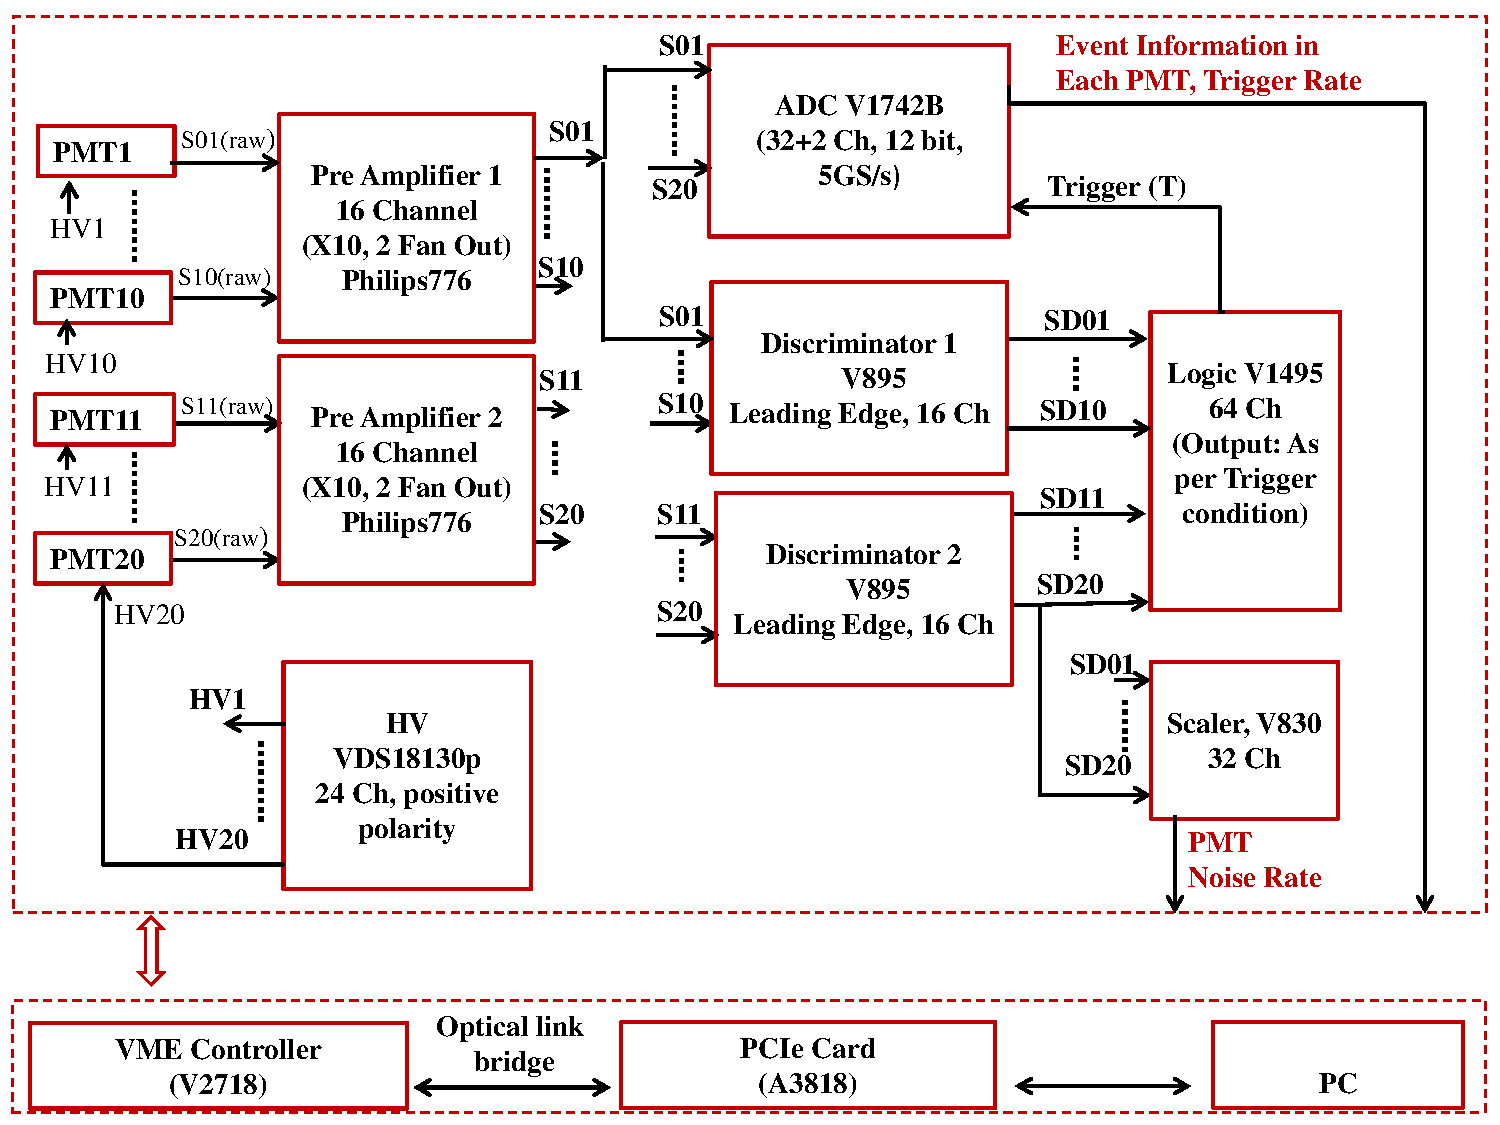
\includegraphics[width=0.85\textwidth]{DAQscheme.pdf}
   \caption{The schematic of the data acquisition system of DireXeno. The 			signal coming from 20 PMTs ({\it i} = 1 -- 20) and the subsequent electronic channels to record the events once triggered. Where S{\it i}(raw) is the raw electrical pulse output of the PMTs, S{\it i} are the amplified pulses, and SD{\it i} are the binary outputs from the discriminator \RanComment{Why is VME controller in lower box }. 
}
   \label{Fig:DAQscheme}
\end{figure}
%%%%%%%%%%%%%%%%%%%%%%%%%%%%%%%%%%%%%%%%%%%%%%%%%%%%%%%%%%%%%%%%%%%%%%%%%%%


The ADC consists of two 12bit 5GS/s switched capacitor digitizer sections, 
each of them with 16+1 channels, based on DRS4 chip. The dynamic range of the input signal is 1 
Vpp with an adjustable DC offset. This module constantly samples (5GS/s, 2.5 GS/s or 2 GS/s) either bipolar or unipolar analog input 
signals, and records them into circular 
analog memory buffers. Once triggered, all analog memory 
buffers are frozen and digitized into a digital memory buffer 
with a 12 bit resolution. 

The binary output signals from the discriminator are duplicated and fed to 

the logic module\footnote{CAEN V1495: FPGA based general purpose VME board} and to a scaler\footnote{CAEN V830: 16 channel scalar}. 
A global majority trigger is generated in the logic module with the coincidence of any two out of the twenty PMTs within a time window of \RanComment{XXX\,ns}. The event information and trigger rate are read from the ADC, while the individual PMTs trigger rate from the scaler. Further analyses of the relevant events are carried out offline.










%\clearpage %temporary TBC
